\documentclass[aspectratio=169]{beamer}
\usetheme{Madrid}
\usecolortheme{beaver}
\usepackage[utf8]{inputenc}
\usepackage[T1]{fontenc}
\usepackage{tikz}
\usepackage{amssymb}
\setbeamertemplate{navigation symbols}{}
\setbeamercolor{title}{fg=white,bg=cyan!60!black}
\setbeamercolor{frametitle}{fg=white,bg=cyan!50!black}
\setbeamercolor{block title}{bg=cyan!15,fg=black}
\setbeamercolor{block body}{bg=cyan!5,fg=black}

\title{G8 — Smart NPCs}
\subtitle{Enemies that chase, flee, patrol; a rule-based chatbot}
\author{ByteForge --- Grade 7 --- Game Maker}
\date{}

\begin{document}

\begin{frame}
    \titlepage
\end{frame}

\begin{frame}{Today's Plan}
    \begin{itemize}
        \item Chase the Player
        \item Patrol Pattern
        \item Rule-Based Chatbot
        \item[$\bigstar$] BOSS --- Enemy with 3 Behaviours
    \end{itemize}
\end{frame}

\begin{frame}{"AI" made entirely of comparisons}
    \Large
    Comparing two positions and nudging one closer, every frame, creates the ILLUSION of hunting — there's no real intelligence, just a repeated comparison.
\end{frame}


\begin{frame}{A direction variable that flips}
    \Large
    Storing "which way" as +1 or -1, flipped at a boundary, creates an endless back-and-forth patrol from one variable and two conditions.

    \begin{center}
    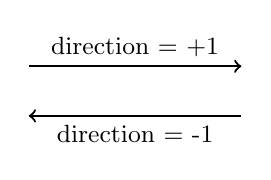
\begin{tikzpicture}[scale=0.9]

        \draw[->, thick] (0,0) -- (3,0);
        \draw[->, thick] (3,-0.7) -- (0,-0.7);
        \node[above] at (1.5,0) {\small direction = +1};
        \node[below] at (1.5,-0.7) {\small direction = -1};
    \end{tikzpicture}
    \end{center}
\end{frame}


\begin{frame}{Matching text — the simplest kind of "AI"}
    \Large
    A rule-based chatbot is just a chain of exact text comparisons, each with its own canned reply — genuinely what early chatbots were.
\end{frame}


\begin{frame}{BOSS — rules vs. real machine learning}
    \Large
    Every behaviour here is a rule YOU wrote. Real ML is different: instead of a human writing rules, the system is shown examples and works out its OWN rules.

    \begin{center}
    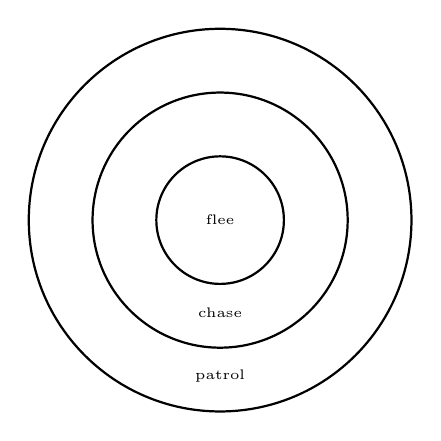
\begin{tikzpicture}[scale=0.9]

        \draw[thick] (0,0) circle (0.9);
        \draw[thick] (0,0) circle (1.8);
        \draw[thick] (0,0) circle (2.7);
        \node at (0,0) {\tiny flee};
        \node at (0,-1.3) {\tiny chase};
        \node at (0,-2.2) {\tiny patrol};
    \end{tikzpicture}
    \end{center}
\end{frame}

\begin{frame}{Real-World Example}
    \Large
    An automated customer-service chat that only understands exact phrases ("Track my order") and fails on anything slightly different is a real rule-based chatbot, exactly like this chapter's. Minecraft mobs are the clearest real-world version of this whole chapter: zombies chase within a distance (chase), iron golems patrol villages, and a chatbot-style villager only "understands" exact trade offers — all rules, no learning.
\end{frame}

\begin{frame}{Watch}
    \Large
    Suggested video topic: \emph{Rule-based AI vs machine learning explained for beginners}

    \vspace{1em}
    \normalsize
    Search this on YouTube together, or swap in a specific video you've
    already vetted --- do not project an unverified link cold in class.
\end{frame}


\begin{frame}{Let Them Discover (1/2)}
    \Large
    Try a simple customer-service chatbot online (a bank, a shop) and type something slightly unusual. Does it understand, or does it fail and repeat a canned response? What does that tell you about how it's built?
\end{frame}


\begin{frame}{Let Them Discover (2/2)}
    \Large
    Watch a Minecraft zombie or spider from a safe distance, then get close. At roughly what distance does it notice and start chasing? That switch is exactly this chapter's distance-based if/else-if/else.
\end{frame}

\begin{frame}{Your Turn}
    \Large
    Open the student map, find \textbf{G8 — Smart NPCs}, and work through it
    hands-on --- everything you just saw, they now do themselves.
\end{frame}

\end{document}
